%%%%%%%%%%%%%%%%%%%%%%%%%%%%%%%%%%%%%%%%%%%%%%%%%%%%%%%%%%%%%%%%%%%%%%%%%%%%%%
%%%%%%%%%%%%%%%%%%%%%%%%%%%%%%%%%%%%%%%%%%%%%%%%%%%%%%%%%%%%%%%%%%%%%%%%%%%%%%
%%
%% Dokumentace úkolu do předmětů IZP a IUS, 2011.
%%
%% Upravená původní dokumentace od Davida Martinka.
%%%%%%%%%%%%%%%%%%%%%%%%%%%%%%%%%%%%%%%%%%%%%%%%%%%%%%%%%%%%%%%%%%%%%%%%%%%%%%
%%%%%%%%%%%%%%%%%%%%%%%%%%%%%%%%%%%%%%%%%%%%%%%%%%%%%%%%%%%%%%%%%%%%%%%%%%%%%%
\documentclass[12pt,a4paper,titlepage,final]{article}

% cestina a fonty
\usepackage[czech]{babel}
\usepackage[utf8]{inputenc}
% balicky pro odkazy
\usepackage[bookmarksopen,colorlinks,plainpages=false,urlcolor=blue,unicode]{hyperref}
\usepackage{url}
% obrazky
\usepackage[dvipdf]{graphicx}
% velikost stranky
\usepackage[top=3.5cm, left=2.5cm, text={17cm, 24cm}, ignorefoot]{geometry}

\begin{document}

%%%%%%%%%%%%%%%%%%%%%%%%%%%%%%%%%%%%%%%%%%%%%%%%%%%%%%%%%%%%%%%%%%%%%%%%%%%%%%
% titulní strana

\def\author{Jan Wrona}
\def\email{xwrona00@stud.fit.vutbr.cz}
\def\projname{Iterační výpočty}

\begin{titlepage}

% \vspace*{1cm}
\begin{figure}[!h]
  \centering
  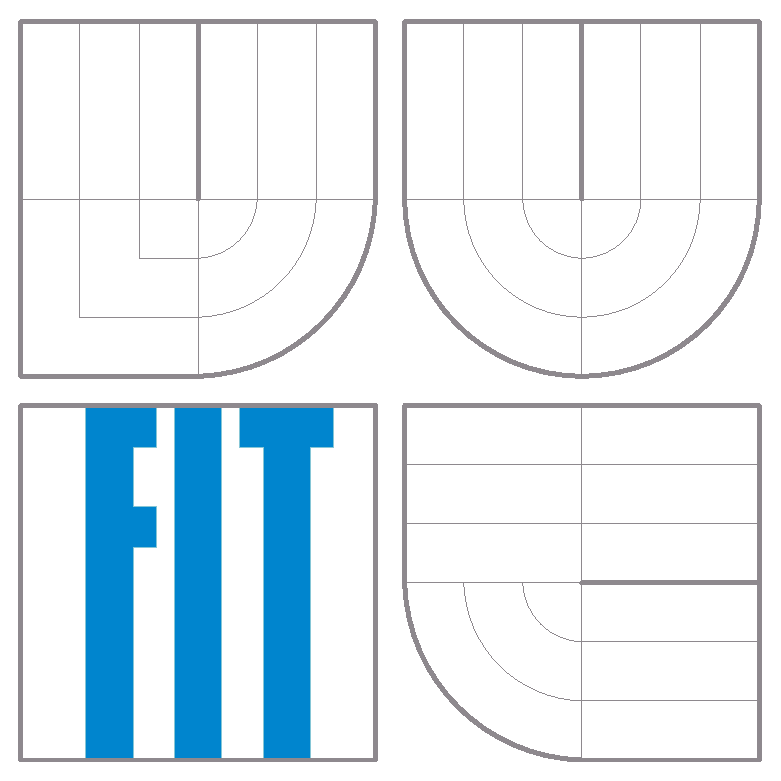
\includegraphics[height=5cm]{img/logo.eps}
\end{figure}

\vfill

\begin{center}
\begin{Large}
Dokumentace k projektu pro předměty IZP a IUS\\
\end{Large}
\bigskip
\begin{Huge}
\projname\\
\end{Huge}
\begin{large}
projekt č. 2
\end{large}
\end{center}

\vfill

\begin{center}
\begin{Large}
\today
\end{Large}
\end{center}

\vfill

\begin{flushleft}
\begin{large}
\begin{tabular}{ll}
Autor: & \author, \url{\email} \\
 & Fakulta Informačních Technologií \\
 & Vysoké Učení Technické v~Brně \\
\end{tabular}
\end{large}
\end{flushleft}
\end{titlepage}


%%%%%%%%%%%%%%%%%%%%%%%%%%%%%%%%%%%%%%%%%%%%%%%%%%%%%%%%%%%%%%%%%%%%%%%%%%%%%%
% obsah
\pagestyle{plain}
\pagenumbering{roman}
\setcounter{page}{1}
\tableofcontents

%%%%%%%%%%%%%%%%%%%%%%%%%%%%%%%%%%%%%%%%%%%%%%%%%%%%%%%%%%%%%%%%%%%%%%%%%%%%%%
% textova zprava
\newpage
\pagestyle{plain}
\pagenumbering{arabic}
\setcounter{page}{1}

%%%%%%%%%%%%%%%%%%%%%%%%%%%%%%%%%%%%%%%%%%%%%%%%%%%%%%%%%%%%%%%%%%%%%%%%%%%%%%
\section{Úvod} \label{uvod}
%%%%%%%%%%%%%%%%%%%%%%%%%%%%%%%%%%%%%%%%%%%%%%%%%%%%%%%%%%%%%%%%%%%%%%%%%%%%%%

Iterační výpočty jsou takové výpočty, které se opakují až do splnění určité
podmínky. Jejich použití v problémech řešených v tomto projektu je klíčové
především z důvodu, že přesný výpočet některých matematických
funkcí může být velmi náročný. V první části projektu jsou tyto výpočty použity
pro aproximaci daných funkcí, ve druhé části pro výpočet průběžné délky lomené
čáry.

Tento dokument popisuje návrh a implementaci aplikace pro výpočet funkce arkus
sinus, logaritmu o zadaném základu, pro výpočet délky lomené čáry a délky
lomené čáry s chybou. Program funguje jako konzolová aplikace, která ze
standardního vstupu čte libovolně dlouhou posloupnost číselných hodnot s plovoucí
řadovou čárkou. Část zajišťijící výpočet funkcí přečte jednu z těchto hodnot
a na standardní výstup vypíše výsledek funkce pro zadanou hodnotu. Část
obstarávající výpočet délky lomené čáry přečtě dvě z těchto hodnot jako
souřadnice a vzhledem k předchozím souřadnicím vypíše průběžnou délku této
čáry, nebo při zadané chybě měření se vypíší minimální a maximální délka čáry.

Dokumentace se skládá z několika částí. V kapitole \ref{analyza} se věnuji analýze
rekurentních problémů, Taylorových řad, také zde objasňuji počítané
matematické funkce arkus sinus a logaritmus. Zaměřuji se i na problematiku
výpočtu délky lomené čáry. Kapitola \ref{navrh} se zabývá obecnými algoritmy
pro aproximaci zadaných funkcí a pro výpočet délky lomené čáry, více potom
pro lomenou čáru s chybou. Součástí této kapitoly je i série testů, které
zkoumají funkci programu i při nesprávném použití. V kapitole
\ref{reseni} mimo jiné objasňuji mou konkrétní implementaci celého programu.
V příloze \ref{metriky} jsou uvedey metriky mého zdrojového kódu a programu.

%%%%%%%%%%%%%%%%%%%%%%%%%%%%%%%%%%%%%%%%%%%%%%%%%%%%%%%%%%%%%%%%%%%%%%%%%%%%%%
\section{Analýza problému a princip jeho řešení} \label{analyza}
%%%%%%%%%%%%%%%%%%%%%%%%%%%%%%%%%%%%%%%%%%%%%%%%%%%%%%%%%%%%%%%%%%%%%%%%%%%%%%

Samotná iterace je, co se implementace týče, problém triviální. Aby ale
iterační výpočet dával nějaký smysl a vedl k rozumným výsledkům v rozumném
čase, musí být vhodně zvoleno tělo  cyklu, tedy ta nejdůležitější část algoritmu,
která vede k správnému výsledku. Nemenší problém je správné zvolení ukončovací
podmínky této iterace. Důležité je samozřejmě také rozumnět všem funkcím,
kterýma se budu v tomto projektu zabývat. Proto se v této kapitole budu věnovat
především analýze těchto problémů.

%=============================================================================
\subsection{Zadání problému}

Cílem tohoto projektu je vytvoření programu v~jazyce C, který pomocí základních
matematických operací aproximuje funkce arkus sinus a logaritmus pro libovolně
dlouhou vstupní posloupnost hodnot. Program musí umět zohlednit přesnost výpočtu
zadávanou jako počet desetinných míst. Druhá část zajišťuje výpočet délky lomené
čáry a lomené čáry s chybou. Chyba je zde zadávána jako absolutní.

%=============================================================================
\subsection{Rekurentní problémy}

Pro aproximaci některých matematických funkcí se často používá
takový druh iterace, při které hodnota aktuálně počítaného kroku závisí až na
několika hodnotách předchozích kroků. Tento speciální případ iterace se nazývá
rekurze a tudíž problémy, které se toho týkají, nazýváme problémy rekurentní
a obecný rekurentní vztah \cite{opora} vypadá následovně:
\begin{equation}\label{eq:rekurentni_vztah}
Y_{n+1} = F(Y_{n}, Y_{n-1}, \dots, Y_{n-k})
\end{equation}
kde Y jsou proměnné vyjadřující hodnotu n-tého kroku a F je funkce pro samotný
výpočet následujícího kroku.
I funkce pro arkus sinus a logaritmus, které jsou řešeny v tomto projektu je možno
aproximovat tímto způsobem, proto se problémem budu dále zabývat.

Jeden z možných způsobů řešení je pomocí nekonečných řad.
To je matematický výraz s obecným vztahem
\begin{equation}\label{eq:nekonecna_rada}
\sum_{n=1}^{\infty }a_{n} = a_{1} + a_{2} + a_{3} + \dots
\end{equation}
kde n je index kroku, a je posloupnost čísel v případě číselné posloupnosti,
ale třeba také funkcí v případě posloupnosti funkční. Z těchto obecných vztahů
lze vyjádřit, pro mé výpočty velmi důležitý, rekurentní vztah pro výpočet
hodnoty následujícího členu řady záviesjícího na hodnotě členu předchozího:
\begin{equation}\label{eq:rekurentni_vztah}
t_{n} = F(t_{n-1}), i>0
\end{equation}
Aby takový rekurentní vztah mohl začít počítat, je potřeba nejprve
inicializovat první člen řady, ať už na nulu, nebo na jakoukoliv jinou
hodnotu dle zvolené řady.


%=============================================================================
\subsection{Taylorovy řady}

Jednou z možností pro aproximaci určitých funkcí je využití Taylorových řad.
Jedná se o zvláštní případ řady mocninné, což je funkční řada, která má ve
svých členech mocninu. Definice Taylorovy řady zní následovně \cite{vzorce}.
V případě existence všech derivací funkce f v bodě a lze Taylorovu řadu zapsat
jako:
\begin{equation}\label{eq:taylorova_rada}
f(x)=\sum_{n=0}^{\infty }a_{n}a^{x}
\end{equation}
Jelikož se jedná a řadu nekonečnou, není možné vyjádřit všechny členy řady, 
a proto se při aproximaci funkce využívá pouze určitý počet členů řady.
Takto upravená Taylorova řada, kde využíváme konečný počet členů řady se nazývá
Taylorův polynom (mnohočlen).

%=============================================================================
\subsection{Funkce arkus sinus}\label{arcsin}

\begin{figure}
  \centering
  % GNUPLOT: LaTeX picture
\setlength{\unitlength}{0.240900pt}
\ifx\plotpoint\undefined\newsavebox{\plotpoint}\fi
\sbox{\plotpoint}{\rule[-0.200pt]{0.400pt}{0.400pt}}%
\begin{picture}(1500,900)(0,0)
\sbox{\plotpoint}{\rule[-0.200pt]{0.400pt}{0.400pt}}%
\put(130.0,100.0){\rule[-0.200pt]{315.338pt}{0.400pt}}
\put(130.0,100.0){\rule[-0.200pt]{4.818pt}{0.400pt}}
\put(110,100){\makebox(0,0)[r]{-1.5}}
\put(1419.0,100.0){\rule[-0.200pt]{4.818pt}{0.400pt}}
\put(130.0,223.0){\rule[-0.200pt]{315.338pt}{0.400pt}}
\put(130.0,223.0){\rule[-0.200pt]{4.818pt}{0.400pt}}
\put(110,223){\makebox(0,0)[r]{-1}}
\put(1419.0,223.0){\rule[-0.200pt]{4.818pt}{0.400pt}}
\put(130.0,347.0){\rule[-0.200pt]{315.338pt}{0.400pt}}
\put(130.0,347.0){\rule[-0.200pt]{4.818pt}{0.400pt}}
\put(110,347){\makebox(0,0)[r]{-0.5}}
\put(1419.0,347.0){\rule[-0.200pt]{4.818pt}{0.400pt}}
\put(130.0,471.0){\rule[-0.200pt]{315.338pt}{0.400pt}}
\put(130.0,471.0){\rule[-0.200pt]{4.818pt}{0.400pt}}
\put(110,471){\makebox(0,0)[r]{ 0}}
\put(1419.0,471.0){\rule[-0.200pt]{4.818pt}{0.400pt}}
\put(130.0,594.0){\rule[-0.200pt]{315.338pt}{0.400pt}}
\put(130.0,594.0){\rule[-0.200pt]{4.818pt}{0.400pt}}
\put(110,594){\makebox(0,0)[r]{ 0.5}}
\put(1419.0,594.0){\rule[-0.200pt]{4.818pt}{0.400pt}}
\put(130.0,718.0){\rule[-0.200pt]{315.338pt}{0.400pt}}
\put(130.0,718.0){\rule[-0.200pt]{4.818pt}{0.400pt}}
\put(110,718){\makebox(0,0)[r]{ 1}}
\put(1419.0,718.0){\rule[-0.200pt]{4.818pt}{0.400pt}}
\put(130.0,841.0){\rule[-0.200pt]{315.338pt}{0.400pt}}
\put(130.0,841.0){\rule[-0.200pt]{4.818pt}{0.400pt}}
\put(110,841){\makebox(0,0)[r]{ 1.5}}
\put(1419.0,841.0){\rule[-0.200pt]{4.818pt}{0.400pt}}
\put(130.0,82.0){\rule[-0.200pt]{0.400pt}{187.179pt}}
\put(130.0,82.0){\rule[-0.200pt]{0.400pt}{4.818pt}}
\put(130,41){\makebox(0,0){-1}}
\put(130.0,839.0){\rule[-0.200pt]{0.400pt}{4.818pt}}
\put(457.0,82.0){\rule[-0.200pt]{0.400pt}{187.179pt}}
\put(457.0,82.0){\rule[-0.200pt]{0.400pt}{4.818pt}}
\put(457,41){\makebox(0,0){-0.5}}
\put(457.0,839.0){\rule[-0.200pt]{0.400pt}{4.818pt}}
\put(785.0,82.0){\rule[-0.200pt]{0.400pt}{187.179pt}}
\put(785.0,82.0){\rule[-0.200pt]{0.400pt}{4.818pt}}
\put(785,41){\makebox(0,0){ 0}}
\put(785.0,839.0){\rule[-0.200pt]{0.400pt}{4.818pt}}
\put(1112.0,82.0){\rule[-0.200pt]{0.400pt}{187.179pt}}
\put(1112.0,82.0){\rule[-0.200pt]{0.400pt}{4.818pt}}
\put(1112,41){\makebox(0,0){ 0.5}}
\put(1112.0,839.0){\rule[-0.200pt]{0.400pt}{4.818pt}}
\put(1439.0,82.0){\rule[-0.200pt]{0.400pt}{187.179pt}}
\put(1439.0,82.0){\rule[-0.200pt]{0.400pt}{4.818pt}}
\put(1439,41){\makebox(0,0){ 1}}
\put(1439.0,839.0){\rule[-0.200pt]{0.400pt}{4.818pt}}
\put(130.0,82.0){\rule[-0.200pt]{0.400pt}{187.179pt}}
\put(130.0,82.0){\rule[-0.200pt]{315.338pt}{0.400pt}}
\put(1439.0,82.0){\rule[-0.200pt]{0.400pt}{187.179pt}}
\put(130.0,859.0){\rule[-0.200pt]{315.338pt}{0.400pt}}
\put(1279,819){\makebox(0,0)[r]{f(x)}}
\put(1299.0,819.0){\rule[-0.200pt]{24.090pt}{0.400pt}}
\put(130,82){\usebox{\plotpoint}}
\multiput(130.58,82.00)(0.493,1.964){23}{\rule{0.119pt}{1.638pt}}
\multiput(129.17,82.00)(13.000,46.599){2}{\rule{0.400pt}{0.819pt}}
\multiput(143.58,132.00)(0.493,0.814){23}{\rule{0.119pt}{0.746pt}}
\multiput(142.17,132.00)(13.000,19.451){2}{\rule{0.400pt}{0.373pt}}
\multiput(156.58,153.00)(0.494,0.570){25}{\rule{0.119pt}{0.557pt}}
\multiput(155.17,153.00)(14.000,14.844){2}{\rule{0.400pt}{0.279pt}}
\multiput(170.00,169.58)(0.497,0.493){23}{\rule{0.500pt}{0.119pt}}
\multiput(170.00,168.17)(11.962,13.000){2}{\rule{0.250pt}{0.400pt}}
\multiput(183.00,182.58)(0.539,0.492){21}{\rule{0.533pt}{0.119pt}}
\multiput(183.00,181.17)(11.893,12.000){2}{\rule{0.267pt}{0.400pt}}
\multiput(196.00,194.58)(0.590,0.492){19}{\rule{0.573pt}{0.118pt}}
\multiput(196.00,193.17)(11.811,11.000){2}{\rule{0.286pt}{0.400pt}}
\multiput(209.00,205.58)(0.704,0.491){17}{\rule{0.660pt}{0.118pt}}
\multiput(209.00,204.17)(12.630,10.000){2}{\rule{0.330pt}{0.400pt}}
\multiput(223.00,215.58)(0.652,0.491){17}{\rule{0.620pt}{0.118pt}}
\multiput(223.00,214.17)(11.713,10.000){2}{\rule{0.310pt}{0.400pt}}
\multiput(236.00,225.59)(0.728,0.489){15}{\rule{0.678pt}{0.118pt}}
\multiput(236.00,224.17)(11.593,9.000){2}{\rule{0.339pt}{0.400pt}}
\multiput(249.00,234.59)(0.824,0.488){13}{\rule{0.750pt}{0.117pt}}
\multiput(249.00,233.17)(11.443,8.000){2}{\rule{0.375pt}{0.400pt}}
\multiput(262.00,242.59)(0.824,0.488){13}{\rule{0.750pt}{0.117pt}}
\multiput(262.00,241.17)(11.443,8.000){2}{\rule{0.375pt}{0.400pt}}
\multiput(275.00,250.59)(0.890,0.488){13}{\rule{0.800pt}{0.117pt}}
\multiput(275.00,249.17)(12.340,8.000){2}{\rule{0.400pt}{0.400pt}}
\multiput(289.00,258.59)(0.950,0.485){11}{\rule{0.843pt}{0.117pt}}
\multiput(289.00,257.17)(11.251,7.000){2}{\rule{0.421pt}{0.400pt}}
\multiput(302.00,265.59)(0.824,0.488){13}{\rule{0.750pt}{0.117pt}}
\multiput(302.00,264.17)(11.443,8.000){2}{\rule{0.375pt}{0.400pt}}
\multiput(315.00,273.59)(0.950,0.485){11}{\rule{0.843pt}{0.117pt}}
\multiput(315.00,272.17)(11.251,7.000){2}{\rule{0.421pt}{0.400pt}}
\multiput(328.00,280.59)(1.026,0.485){11}{\rule{0.900pt}{0.117pt}}
\multiput(328.00,279.17)(12.132,7.000){2}{\rule{0.450pt}{0.400pt}}
\multiput(342.00,287.59)(1.123,0.482){9}{\rule{0.967pt}{0.116pt}}
\multiput(342.00,286.17)(10.994,6.000){2}{\rule{0.483pt}{0.400pt}}
\multiput(355.00,293.59)(0.950,0.485){11}{\rule{0.843pt}{0.117pt}}
\multiput(355.00,292.17)(11.251,7.000){2}{\rule{0.421pt}{0.400pt}}
\multiput(368.00,300.59)(1.123,0.482){9}{\rule{0.967pt}{0.116pt}}
\multiput(368.00,299.17)(10.994,6.000){2}{\rule{0.483pt}{0.400pt}}
\multiput(381.00,306.59)(0.950,0.485){11}{\rule{0.843pt}{0.117pt}}
\multiput(381.00,305.17)(11.251,7.000){2}{\rule{0.421pt}{0.400pt}}
\multiput(394.00,313.59)(1.214,0.482){9}{\rule{1.033pt}{0.116pt}}
\multiput(394.00,312.17)(11.855,6.000){2}{\rule{0.517pt}{0.400pt}}
\multiput(408.00,319.59)(1.123,0.482){9}{\rule{0.967pt}{0.116pt}}
\multiput(408.00,318.17)(10.994,6.000){2}{\rule{0.483pt}{0.400pt}}
\multiput(421.00,325.59)(1.123,0.482){9}{\rule{0.967pt}{0.116pt}}
\multiput(421.00,324.17)(10.994,6.000){2}{\rule{0.483pt}{0.400pt}}
\multiput(434.00,331.59)(1.123,0.482){9}{\rule{0.967pt}{0.116pt}}
\multiput(434.00,330.17)(10.994,6.000){2}{\rule{0.483pt}{0.400pt}}
\multiput(447.00,337.59)(1.489,0.477){7}{\rule{1.220pt}{0.115pt}}
\multiput(447.00,336.17)(11.468,5.000){2}{\rule{0.610pt}{0.400pt}}
\multiput(461.00,342.59)(1.123,0.482){9}{\rule{0.967pt}{0.116pt}}
\multiput(461.00,341.17)(10.994,6.000){2}{\rule{0.483pt}{0.400pt}}
\multiput(474.00,348.59)(1.123,0.482){9}{\rule{0.967pt}{0.116pt}}
\multiput(474.00,347.17)(10.994,6.000){2}{\rule{0.483pt}{0.400pt}}
\multiput(487.00,354.59)(1.378,0.477){7}{\rule{1.140pt}{0.115pt}}
\multiput(487.00,353.17)(10.634,5.000){2}{\rule{0.570pt}{0.400pt}}
\multiput(500.00,359.59)(1.123,0.482){9}{\rule{0.967pt}{0.116pt}}
\multiput(500.00,358.17)(10.994,6.000){2}{\rule{0.483pt}{0.400pt}}
\multiput(513.00,365.59)(1.489,0.477){7}{\rule{1.220pt}{0.115pt}}
\multiput(513.00,364.17)(11.468,5.000){2}{\rule{0.610pt}{0.400pt}}
\multiput(527.00,370.59)(1.123,0.482){9}{\rule{0.967pt}{0.116pt}}
\multiput(527.00,369.17)(10.994,6.000){2}{\rule{0.483pt}{0.400pt}}
\multiput(540.00,376.59)(1.378,0.477){7}{\rule{1.140pt}{0.115pt}}
\multiput(540.00,375.17)(10.634,5.000){2}{\rule{0.570pt}{0.400pt}}
\multiput(553.00,381.59)(1.378,0.477){7}{\rule{1.140pt}{0.115pt}}
\multiput(553.00,380.17)(10.634,5.000){2}{\rule{0.570pt}{0.400pt}}
\multiput(566.00,386.59)(1.214,0.482){9}{\rule{1.033pt}{0.116pt}}
\multiput(566.00,385.17)(11.855,6.000){2}{\rule{0.517pt}{0.400pt}}
\multiput(580.00,392.59)(1.378,0.477){7}{\rule{1.140pt}{0.115pt}}
\multiput(580.00,391.17)(10.634,5.000){2}{\rule{0.570pt}{0.400pt}}
\multiput(593.00,397.59)(1.378,0.477){7}{\rule{1.140pt}{0.115pt}}
\multiput(593.00,396.17)(10.634,5.000){2}{\rule{0.570pt}{0.400pt}}
\multiput(606.00,402.59)(1.378,0.477){7}{\rule{1.140pt}{0.115pt}}
\multiput(606.00,401.17)(10.634,5.000){2}{\rule{0.570pt}{0.400pt}}
\multiput(619.00,407.59)(1.123,0.482){9}{\rule{0.967pt}{0.116pt}}
\multiput(619.00,406.17)(10.994,6.000){2}{\rule{0.483pt}{0.400pt}}
\multiput(632.00,413.59)(1.489,0.477){7}{\rule{1.220pt}{0.115pt}}
\multiput(632.00,412.17)(11.468,5.000){2}{\rule{0.610pt}{0.400pt}}
\multiput(646.00,418.59)(1.378,0.477){7}{\rule{1.140pt}{0.115pt}}
\multiput(646.00,417.17)(10.634,5.000){2}{\rule{0.570pt}{0.400pt}}
\multiput(659.00,423.59)(1.378,0.477){7}{\rule{1.140pt}{0.115pt}}
\multiput(659.00,422.17)(10.634,5.000){2}{\rule{0.570pt}{0.400pt}}
\multiput(672.00,428.59)(1.378,0.477){7}{\rule{1.140pt}{0.115pt}}
\multiput(672.00,427.17)(10.634,5.000){2}{\rule{0.570pt}{0.400pt}}
\multiput(685.00,433.59)(1.489,0.477){7}{\rule{1.220pt}{0.115pt}}
\multiput(685.00,432.17)(11.468,5.000){2}{\rule{0.610pt}{0.400pt}}
\multiput(699.00,438.59)(1.378,0.477){7}{\rule{1.140pt}{0.115pt}}
\multiput(699.00,437.17)(10.634,5.000){2}{\rule{0.570pt}{0.400pt}}
\multiput(712.00,443.59)(1.378,0.477){7}{\rule{1.140pt}{0.115pt}}
\multiput(712.00,442.17)(10.634,5.000){2}{\rule{0.570pt}{0.400pt}}
\multiput(725.00,448.59)(1.378,0.477){7}{\rule{1.140pt}{0.115pt}}
\multiput(725.00,447.17)(10.634,5.000){2}{\rule{0.570pt}{0.400pt}}
\multiput(738.00,453.59)(1.378,0.477){7}{\rule{1.140pt}{0.115pt}}
\multiput(738.00,452.17)(10.634,5.000){2}{\rule{0.570pt}{0.400pt}}
\multiput(751.00,458.59)(1.489,0.477){7}{\rule{1.220pt}{0.115pt}}
\multiput(751.00,457.17)(11.468,5.000){2}{\rule{0.610pt}{0.400pt}}
\multiput(765.00,463.59)(1.378,0.477){7}{\rule{1.140pt}{0.115pt}}
\multiput(765.00,462.17)(10.634,5.000){2}{\rule{0.570pt}{0.400pt}}
\multiput(778.00,468.59)(1.378,0.477){7}{\rule{1.140pt}{0.115pt}}
\multiput(778.00,467.17)(10.634,5.000){2}{\rule{0.570pt}{0.400pt}}
\multiput(791.00,473.59)(1.378,0.477){7}{\rule{1.140pt}{0.115pt}}
\multiput(791.00,472.17)(10.634,5.000){2}{\rule{0.570pt}{0.400pt}}
\multiput(804.00,478.59)(1.489,0.477){7}{\rule{1.220pt}{0.115pt}}
\multiput(804.00,477.17)(11.468,5.000){2}{\rule{0.610pt}{0.400pt}}
\multiput(818.00,483.59)(1.378,0.477){7}{\rule{1.140pt}{0.115pt}}
\multiput(818.00,482.17)(10.634,5.000){2}{\rule{0.570pt}{0.400pt}}
\multiput(831.00,488.59)(1.378,0.477){7}{\rule{1.140pt}{0.115pt}}
\multiput(831.00,487.17)(10.634,5.000){2}{\rule{0.570pt}{0.400pt}}
\multiput(844.00,493.59)(1.378,0.477){7}{\rule{1.140pt}{0.115pt}}
\multiput(844.00,492.17)(10.634,5.000){2}{\rule{0.570pt}{0.400pt}}
\multiput(857.00,498.59)(1.378,0.477){7}{\rule{1.140pt}{0.115pt}}
\multiput(857.00,497.17)(10.634,5.000){2}{\rule{0.570pt}{0.400pt}}
\multiput(870.00,503.59)(1.489,0.477){7}{\rule{1.220pt}{0.115pt}}
\multiput(870.00,502.17)(11.468,5.000){2}{\rule{0.610pt}{0.400pt}}
\multiput(884.00,508.59)(1.378,0.477){7}{\rule{1.140pt}{0.115pt}}
\multiput(884.00,507.17)(10.634,5.000){2}{\rule{0.570pt}{0.400pt}}
\multiput(897.00,513.59)(1.378,0.477){7}{\rule{1.140pt}{0.115pt}}
\multiput(897.00,512.17)(10.634,5.000){2}{\rule{0.570pt}{0.400pt}}
\multiput(910.00,518.59)(1.378,0.477){7}{\rule{1.140pt}{0.115pt}}
\multiput(910.00,517.17)(10.634,5.000){2}{\rule{0.570pt}{0.400pt}}
\multiput(923.00,523.59)(1.489,0.477){7}{\rule{1.220pt}{0.115pt}}
\multiput(923.00,522.17)(11.468,5.000){2}{\rule{0.610pt}{0.400pt}}
\multiput(937.00,528.59)(1.123,0.482){9}{\rule{0.967pt}{0.116pt}}
\multiput(937.00,527.17)(10.994,6.000){2}{\rule{0.483pt}{0.400pt}}
\multiput(950.00,534.59)(1.378,0.477){7}{\rule{1.140pt}{0.115pt}}
\multiput(950.00,533.17)(10.634,5.000){2}{\rule{0.570pt}{0.400pt}}
\multiput(963.00,539.59)(1.378,0.477){7}{\rule{1.140pt}{0.115pt}}
\multiput(963.00,538.17)(10.634,5.000){2}{\rule{0.570pt}{0.400pt}}
\multiput(976.00,544.59)(1.378,0.477){7}{\rule{1.140pt}{0.115pt}}
\multiput(976.00,543.17)(10.634,5.000){2}{\rule{0.570pt}{0.400pt}}
\multiput(989.00,549.59)(1.214,0.482){9}{\rule{1.033pt}{0.116pt}}
\multiput(989.00,548.17)(11.855,6.000){2}{\rule{0.517pt}{0.400pt}}
\multiput(1003.00,555.59)(1.378,0.477){7}{\rule{1.140pt}{0.115pt}}
\multiput(1003.00,554.17)(10.634,5.000){2}{\rule{0.570pt}{0.400pt}}
\multiput(1016.00,560.59)(1.378,0.477){7}{\rule{1.140pt}{0.115pt}}
\multiput(1016.00,559.17)(10.634,5.000){2}{\rule{0.570pt}{0.400pt}}
\multiput(1029.00,565.59)(1.123,0.482){9}{\rule{0.967pt}{0.116pt}}
\multiput(1029.00,564.17)(10.994,6.000){2}{\rule{0.483pt}{0.400pt}}
\multiput(1042.00,571.59)(1.489,0.477){7}{\rule{1.220pt}{0.115pt}}
\multiput(1042.00,570.17)(11.468,5.000){2}{\rule{0.610pt}{0.400pt}}
\multiput(1056.00,576.59)(1.123,0.482){9}{\rule{0.967pt}{0.116pt}}
\multiput(1056.00,575.17)(10.994,6.000){2}{\rule{0.483pt}{0.400pt}}
\multiput(1069.00,582.59)(1.378,0.477){7}{\rule{1.140pt}{0.115pt}}
\multiput(1069.00,581.17)(10.634,5.000){2}{\rule{0.570pt}{0.400pt}}
\multiput(1082.00,587.59)(1.123,0.482){9}{\rule{0.967pt}{0.116pt}}
\multiput(1082.00,586.17)(10.994,6.000){2}{\rule{0.483pt}{0.400pt}}
\multiput(1095.00,593.59)(1.123,0.482){9}{\rule{0.967pt}{0.116pt}}
\multiput(1095.00,592.17)(10.994,6.000){2}{\rule{0.483pt}{0.400pt}}
\multiput(1108.00,599.59)(1.489,0.477){7}{\rule{1.220pt}{0.115pt}}
\multiput(1108.00,598.17)(11.468,5.000){2}{\rule{0.610pt}{0.400pt}}
\multiput(1122.00,604.59)(1.123,0.482){9}{\rule{0.967pt}{0.116pt}}
\multiput(1122.00,603.17)(10.994,6.000){2}{\rule{0.483pt}{0.400pt}}
\multiput(1135.00,610.59)(1.123,0.482){9}{\rule{0.967pt}{0.116pt}}
\multiput(1135.00,609.17)(10.994,6.000){2}{\rule{0.483pt}{0.400pt}}
\multiput(1148.00,616.59)(1.123,0.482){9}{\rule{0.967pt}{0.116pt}}
\multiput(1148.00,615.17)(10.994,6.000){2}{\rule{0.483pt}{0.400pt}}
\multiput(1161.00,622.59)(1.214,0.482){9}{\rule{1.033pt}{0.116pt}}
\multiput(1161.00,621.17)(11.855,6.000){2}{\rule{0.517pt}{0.400pt}}
\multiput(1175.00,628.59)(0.950,0.485){11}{\rule{0.843pt}{0.117pt}}
\multiput(1175.00,627.17)(11.251,7.000){2}{\rule{0.421pt}{0.400pt}}
\multiput(1188.00,635.59)(1.123,0.482){9}{\rule{0.967pt}{0.116pt}}
\multiput(1188.00,634.17)(10.994,6.000){2}{\rule{0.483pt}{0.400pt}}
\multiput(1201.00,641.59)(0.950,0.485){11}{\rule{0.843pt}{0.117pt}}
\multiput(1201.00,640.17)(11.251,7.000){2}{\rule{0.421pt}{0.400pt}}
\multiput(1214.00,648.59)(1.123,0.482){9}{\rule{0.967pt}{0.116pt}}
\multiput(1214.00,647.17)(10.994,6.000){2}{\rule{0.483pt}{0.400pt}}
\multiput(1227.00,654.59)(1.026,0.485){11}{\rule{0.900pt}{0.117pt}}
\multiput(1227.00,653.17)(12.132,7.000){2}{\rule{0.450pt}{0.400pt}}
\multiput(1241.00,661.59)(0.950,0.485){11}{\rule{0.843pt}{0.117pt}}
\multiput(1241.00,660.17)(11.251,7.000){2}{\rule{0.421pt}{0.400pt}}
\multiput(1254.00,668.59)(0.824,0.488){13}{\rule{0.750pt}{0.117pt}}
\multiput(1254.00,667.17)(11.443,8.000){2}{\rule{0.375pt}{0.400pt}}
\multiput(1267.00,676.59)(0.950,0.485){11}{\rule{0.843pt}{0.117pt}}
\multiput(1267.00,675.17)(11.251,7.000){2}{\rule{0.421pt}{0.400pt}}
\multiput(1280.00,683.59)(0.890,0.488){13}{\rule{0.800pt}{0.117pt}}
\multiput(1280.00,682.17)(12.340,8.000){2}{\rule{0.400pt}{0.400pt}}
\multiput(1294.00,691.59)(0.824,0.488){13}{\rule{0.750pt}{0.117pt}}
\multiput(1294.00,690.17)(11.443,8.000){2}{\rule{0.375pt}{0.400pt}}
\multiput(1307.00,699.59)(0.824,0.488){13}{\rule{0.750pt}{0.117pt}}
\multiput(1307.00,698.17)(11.443,8.000){2}{\rule{0.375pt}{0.400pt}}
\multiput(1320.00,707.59)(0.728,0.489){15}{\rule{0.678pt}{0.118pt}}
\multiput(1320.00,706.17)(11.593,9.000){2}{\rule{0.339pt}{0.400pt}}
\multiput(1333.00,716.58)(0.652,0.491){17}{\rule{0.620pt}{0.118pt}}
\multiput(1333.00,715.17)(11.713,10.000){2}{\rule{0.310pt}{0.400pt}}
\multiput(1346.00,726.58)(0.704,0.491){17}{\rule{0.660pt}{0.118pt}}
\multiput(1346.00,725.17)(12.630,10.000){2}{\rule{0.330pt}{0.400pt}}
\multiput(1360.00,736.58)(0.590,0.492){19}{\rule{0.573pt}{0.118pt}}
\multiput(1360.00,735.17)(11.811,11.000){2}{\rule{0.286pt}{0.400pt}}
\multiput(1373.00,747.58)(0.539,0.492){21}{\rule{0.533pt}{0.119pt}}
\multiput(1373.00,746.17)(11.893,12.000){2}{\rule{0.267pt}{0.400pt}}
\multiput(1386.00,759.58)(0.497,0.493){23}{\rule{0.500pt}{0.119pt}}
\multiput(1386.00,758.17)(11.962,13.000){2}{\rule{0.250pt}{0.400pt}}
\multiput(1399.58,772.00)(0.494,0.570){25}{\rule{0.119pt}{0.557pt}}
\multiput(1398.17,772.00)(14.000,14.844){2}{\rule{0.400pt}{0.279pt}}
\multiput(1413.58,788.00)(0.493,0.814){23}{\rule{0.119pt}{0.746pt}}
\multiput(1412.17,788.00)(13.000,19.451){2}{\rule{0.400pt}{0.373pt}}
\multiput(1426.58,809.00)(0.493,1.964){23}{\rule{0.119pt}{1.638pt}}
\multiput(1425.17,809.00)(13.000,46.599){2}{\rule{0.400pt}{0.819pt}}
\put(130.0,82.0){\rule[-0.200pt]{0.400pt}{187.179pt}}
\put(130.0,82.0){\rule[-0.200pt]{315.338pt}{0.400pt}}
\put(1439.0,82.0){\rule[-0.200pt]{0.400pt}{187.179pt}}
\put(130.0,859.0){\rule[-0.200pt]{315.338pt}{0.400pt}}
\end{picture}

  \caption{Graf funkce arkus sinus}
  \label{fig:arkus_sinus}
\end{figure}

Arkus sinus (značená též jako arcsin, asin) je funkce cyklometrická, tzn. 
funkce inverzní k funkci goniomterické. V tomto případě tedy hovořím o 
funkci arkus sinus, která je inverzní k sinus a naopak.
Definiční obor funkce je $\langle-1, 1\rangle$, obor hodnot je 
$\langle-\frac{\pi}{2},\frac{\pi}{2}\rangle$.
Funkci arkus sinus, tak jako jiné cyklometrické funkce, lze vyjádřit pomocí
jiných cyklometrických funkcí stejného argumentu \cite{vzorce}:
\begin{equation}\label{eq:arcsin_arccos}
arcsin(x) = \frac{\pi}{2}-arccos(x)
\end{equation}
pro definiční obor $(|x|\le 1)$, nebo také:
\begin{equation}\label{eq:arcsin_arctan}
arcsin(x) = arctan\frac{x}{\sqrt{(1-x^2)}}
\end{equation}
pro definiční obor $(|x|<1)$.
Graf cyklometrických lze sestrojit z grafů goniometrických funkcí na
intervalech, kde jsou monotónní. Funkce sinus je monotónní v intervalu
$\langle-\frac{\pi}{2}, \frac{\pi}{2}\rangle$, graf funkce arkus sinus
znázorňuje obrázek \ref{fig:arkus_sinus}

%=============================================================================
\subsection{Funkce logaritmus}

Logaritmus je matematická funkce inverzní k funkci exponenciální.
Logaritmus zapisujeme jako
\begin{equation}\label{eq:logaritmus}
y=\log_{a}x
\end{equation}
kde x je logaritmované číslo (někdy také numerus) a číslo a
($a\in R^{+}-\{1\}$) označuje zálkad logaritmu (někdy také báze). Logaritmus
o základu 10 nazýváme desítkový (značíme ho $\log_{}x$, desítka se často nepíše),
o základu $e$\footnote{Eulerovo číslo,
jeho hodnorta je 2,71828\dots} nazýváme přirozený (ten je také možno
značit jako $\ln_{}x$).
Je možno odvodit a zjistit spoustu různých vlastností a vztahů pro logaritmus, 
uvedu zde ale jen ty pro můj projekt podstatné, jako například tento vztah \cite{tabulky}
pro vyjádření logaritmu o jakémkoliv základu pomocí dvou desítkových nebo
přirozených logaritmů:
\begin{equation}\label{eq:logaritmus2}
\log_{a}x=\frac{\log_{}x}{\log_{}a}=\frac{\ln_{}x}{\ln_{}a}
\end{equation}
Pokud přepočítáme číslo jako mantisu m o exponentu e, lze desítkový logaritmus
vyjádřit pomocí tohoto vztahu:
\begin{equation}\label{eq:logaritmus3}
\log_{}x=\log_{m}+e
\end{equation}

%=============================================================================
\subsection{Lomená čára}

\begin{figure}
  \centering
  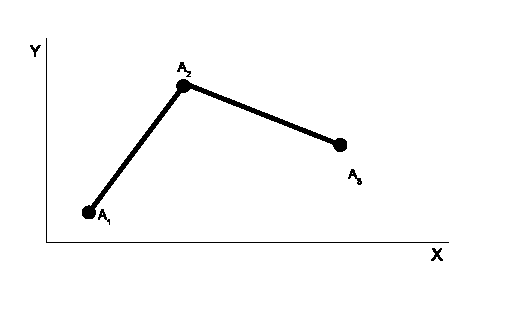
\includegraphics{img/lomcara.eps}
  \caption{Lomená čára}
  \label{fig:lomena_cara}
\end{figure}

Lomená čára je spojená série úseček. Pokud máme v rovině body ($A_1,A_2,\dots,
A_n$), tak úsečky jejichž koncové body jsou počátečními body dalších úseček
($A_1A_2, A_2A_3,\dots,A_{n-1}A_n$) tvoří lomenou čáru.
Pro představu uvádím příklad lomené čáry na obrázku \ref{fig:lomena_cara}.


%=============================================================================
\subsection{Lomená čára s chybou}

Lomená čára s chybou je v podstatě totožná s klasickou lomenou čárou.
Rozdíl je ten, že po zohlednění této chyby se už nebude jednat o body v rovině,
ale o množinu bodů, a pokud by chyba byla zadána totožně pro obě souřadnice, 
jednalo by se o množinu představující čtverec. Jak plyne z obrázku
\ref{fig:lomena_cara_ch}, po aplikaci této chyby vznikne nekonečný počet
lomených čar, budu se zde ale zabývat pouze tou s nejmenší možnou a největší
možnou délkou.

\begin{figure}
  \centering
  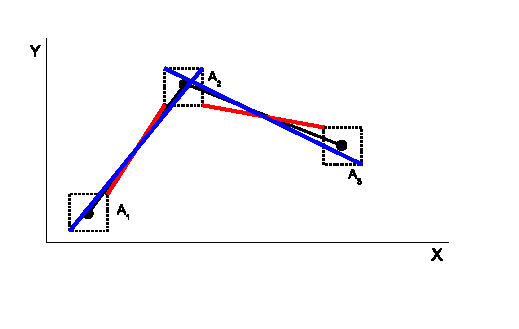
\includegraphics{img/lomcara_ch.eps}
  \caption{Lomená čára s chybou. Černou barvou je vykreslena původní čára bez
           chyby, červenou čárou nejkratší možná délka a modrou je vykreslena
           nejdelší možná délka čáry.}
  \label{fig:lomena_cara_ch}
\end{figure}

%=============================================================================
\subsection{Rozsah hodnot}

Rozsah vstupních hodnot je v případě obou funkcí jasný. U arkus sinus
se jedná o definiční obor této funkce, který je v uveden v podkapitole
\ref{arcsin}. Také logaritmus je definován pouze pro hodnoty větší než nula a
základ logaritmu mohou být pouze kladná reálná čísla vyjma jedničky. U vstupních
hodnot pro lomené čáry platí omezení pouze rozsahem použitého datového typu.

%%%%%%%%%%%%%%%%%%%%%%%%%%%%%%%%%%%%%%%%%%%%%%%%%%%%%%%%%%%%%%%%%%%%%%%%%%%%%%
\newpage
\section{Návrh řešení problému} \label{navrh}
%%%%%%%%%%%%%%%%%%%%%%%%%%%%%%%%%%%%%%%%%%%%%%%%%%%%%%%%%%%%%%%%%%%%%%%%%%%%%%


%=============================================================================
\subsection{Volba datových typů}

U veškerých proměnných s plovoucí řadovou čárkou jsem zvoli datový typ \texttt{double}
z důvodu většího rozsahu možných hodnot. Vstupní hodnoty je tedy možno zadávat
v rozsahu přibližně $1.7e^{\pm308}$. Stejný rozsah platí i pro hodnoty výsledné.
U proměnných bez plovoucí řadové čárky jsem volil datový typ \texttt{int}. S takovýma
proměnnýma se v tomto programu neprovádí žádné zásadní výpočty, jedná se tedy
většinou o různé pomocné proměnné u kterých rozsah není podstatný.

%=============================================================================
\subsection{Výpočet arkus sinus}

Pro aproximaci funkce arkus sinus jsem zvolil jedno z možných vyjádření této
funkce pomocí funkce jiné. Jedná se konkrétně o vztah \ref{eq:arcsin_arctan}.
Jak je také uvedeno v podkapitole \ref{arcsin}, tento vztah je možné využít
pouze pro aproximaci hodnot v intervalu $(-1, 1)$, kdežto definiční obor funce
arkus sinus je $\langle-1,1\rangle$. Proto je nutné zohlednit případy, kdy je
požadován výpočet funkce s parametrem 1 nebo -1. Pro aproximaci arkus sinus
je tedy potřeba aproximovat funkci arkus tanges a upravit její parametr.
Proto budu nyní popisovat realizaci funce arkus tangens. Taylorův rozvoj pro
výpočet arkus tangens \cite{vzorce}
\begin{equation}\label{eq:taylor_tangens}
\sum_{n=0}^{\infty }(-1)^{n}\frac{x^{2n-1}}{2n+1}
\end{equation}
jsem upravil tak, aby každý další krok mohl být vyjádřen rekurentně pomocí
předchozího kroku:
\begin{equation}\label{eq:rekur_tangens}
t_{n}=t_{n-1}\cdot (-\frac{x^{2}(n-1)}{n+1})
\end{equation}
Tímto se podstatně sníží náročnost výpočtu jednoho kroku. První krok je potřeba
inicializovat, u tohoto Taylorova rozvoje je hodnota prvního kroku shodná s
hodnotou zadanáho parametru. Postupný součet jednotlivých kroků se ukládá
do proměnné. Tento rekurentní vztah se tedy opakuje v cyklu s ukončovací
podmínkou, kterou rozebírám v samostatné podkapitole \ref{podminka}.
Vzhledem k této Taylorově řadě jsem z důvodů zvýšení efektivity algoritmu
upravil zadaný parametr dvěma způsoby. Když je záporný, tak se neguje,
algoritmus počítá s číslem kladným a neguje se až výsledek. Další úprava
invertuje parametr, pokud je větší než 1 a výpočítaný výsledek odečte od
$\frac{\pi}{2}$.

%=============================================================================
\subsection{Výpočet logaritmu}

Pro výpočet přirozeného logaritmu jsem zvolil vztah \ref{eq:logaritmus2},
takže nadále budu popisovat funkci, která aproximuje přirozený logaritmus.
V rámci heuristiky je nejprve potřeba patřičně upravit zadané
logaritmované číslo. To se provede jeho rozdělením na exponent a mantisu tak,
aby mantisa ležela vždy v intervalu $\langle1,10\rangle$,
přičemž se s těmito čísly nadále pracuje podle vztahu \ref{eq:logaritmus3}.
Tento vztah je pro desítkový logaritmus, můj algoritmus ale počítá přirozený
logaritmus, proto jsem si tento vztah patřičně upravil:
\begin{equation}\label{eq:taylor_logaritmus}
ln(x)=ln(m)+e\cdot ln(10)
\end{equation}
Logaritmus má omezený definiční obor, je tedy potřeba ošetřit hodnoty
logarotmových čísel ležících mimo definiční obor pomocí hodnot NAN a INFINITY.
Taylorův rozvoj pro přirozený logaritmus
\begin{equation}\label{eq:taylor_logaritmus}
\sum_{n=1}^{\infty }\frac{(-1)^{n+1}}{n}\cdot (x-1)^{n}
\end{equation}
jsem upravil do podoby rekurentního vztahu:
\begin{equation}\label{eq:rekus_logaritmus}
t_{n}=t_{n-1}\cdot (\frac{(1-n)(x-1)}{n})
\end{equation}
Inicializace prvního kroku zde podle Taylorovy řady bude $x-1$. Tento Taylorův
rozvoj ale poskytuje přesnou aproximaci pouze v intervalu $(0,2\rangle$, proto
je pro výpočet logaritmu většího než 2 je řada přepočítaná pomocí Eulerovy
transformace do podoby:
\begin{equation}\label{eq:taylor_logaritmus2}
ln\frac{x}{x-1}=\sum_{n=1}^{\infty }\frac{1}{nx^{n}}
\end{equation}
Aby ale počítal pro zadané logaritmové číslo x a ne pro $\frac{x}{x-1}$, 
je potřeba upravit x do podoby $\frac{x}{x-1}$, potom po dosazení:
\begin{equation}
\frac{\frac{x}{x-1}}{\frac{x}{x-1}-1}=x
\end{equation}
Vztah \ref{eq:taylor_logaritmus2} vyjádřený rekurentně vypadá následovně:
\begin{equation}
t_{n} = t_{n-1}\cdot (\frac{n-1}{nx})
\end{equation}
kde inicializace prvního kroku bude $\frac{1}{x}$. Oba dva tyto rekurentní
vztahy jsou umístěny v cyklech s ukončovací podmínkou, kterou rozebírám v
samostatné podkapitole \ref{podminka}.

%============================================================================
\subsection{Ukončovací podmínka iteračních výpočtů}\label{podminka}

Požadovaná přesnost u arkus sinus a logaritmu je v tomto projektu zadávána
relativně. S ohledem na to, že Taylorovy řady nejsou pro celý definiční obor
stejně přesné, počet iterací nebude pro každou vstupní hodnotu stejný.
Ukončovací podmínku tedy není možné zadat jako pevný počet iterací, ale musí
být také zadána relativně, relativně vzhledem k výsledku.

Jedno z možných řešení tohoto problému je umístit do podmínky tento vztah:
\begin{equation}\label{eq:podminka}
|t_{n}|>|\sum_{}^{}t|*sigdig
\end{equation}
Přesnost sigdig zadaná jako počet desetinných míst by se ale do tohoto vzahu
nehodila, proto se musí přepočítat jako $10^{-sigdig}$.

%=============================================================================
\subsection{Výpočet délky lomené čáry a lomené čáry s chybou}

Jak je zmíněno v analýze, lomená čára je série úseček. Proto pro výpočet její
délky je potřeba znát délky těchto úseček. Jednu úsečku v rovině si lze
představit jako přeponu trojuhelníku.
Výpočtem rozdílu zadaných souřadnic lze získat délku jeho odvěsen, a přeponu 
tedy vypočítáme pomocí Pythagorovy věty $c^2=a^2+b^2$. Součet jednotlivých
přenom je roven délce lomené čáry.

U lomené čáry s chybou je situace komplikovanější. Nejprve je potřeba vytvořit
intervaly možných hodnot souřadnic, to se provede odečtením/přičtením chyby
od/ke každé souřadnici. Pro získání nejmenší
a největší vzdálenosti těchto intervalů jsem použil vztah intervalové
aritmetiky pro odečítání:
\begin{equation}\label{eq:inetvalova_aritmetika}
(a,b)-(c,d)=(a-d,b-c)
\end{equation}
který jsem pro své potřeby upravil jako:
\begin{equation}\label{eq:inetvalova_aritmetika}
(a,b)-(c,d)=(d-a,c-b)
\end{equation}
Tuto intervalovou aritmetiku provádím s intervaly vzniklými aplikací chyby
na vstupní souřadnice. Výsledné dva intervaly určují největší a nejmenší
vzdálenost těchto intervalů podle osy x a y. Následná nejkratší a nejdelší
úsečka se z těchto hodnot vypočítá pomocí Pythagorovy věty. Mohou ale nastat
určité situace, při kterých je výsledek jiný. Pokud jsou obě nejmenší délky
(jak pro x tak pro y) menší než 0, budou se pomyslné čtverce překrývat a
nejmenší chyba bude~0\footnote{Bez tohoto ošetření by mohla vzniknout lomená
čára o záporné délce.}. Pokud bude alespoň jedna z nejmenších délek menší než 0,
překrývají se intervaly pouze podle jedné osy a nejmenší délka tudíž není
vzálenost rohů těchto pomyslných čtverců, ale vzdálenost jejich bližších stran.

%=============================================================================
\subsection{Specifikace testů} \label{testy}

Z~návrhu řešení vyplývá několik rizikových oblastí, které je potřeba otestovat,
jako například chybný rozsah vstupních hodnot, chybně zadaná chyba či přesnost
pomocí příkazové řádky, vstupní hodnota mimo definiční obor funkce nebo vstupní
hodnota větší než je rozsah datového typu \texttt{double}.

\paragraph{Test 1:} Chybně zadaná přesnost sigdig $\longrightarrow$ Detekce chyby.
\begin{verbatim}
-3
3a
abc
\end{verbatim} 

\paragraph{Test 2:} Chybně zadaná chyba ERR $\longrightarrow$ Detekce chyby.
\begin{verbatim}
-4
4b
def
\end{verbatim} 

\paragraph{Test 3:} Základ logaritmu neodpovídá definici $\longrightarrow$ Výpis
NAN
\begin{verbatim}
-2
-45
\end{verbatim} 

\paragraph{Test 4:} Chybně zadaný základ logaritmu $\longrightarrow$ Detekce
chyby.
\begin{verbatim}
a
-3s
ghk
\end{verbatim}

\paragraph{Test 5:} Vstupní data přesahující rozsah datového typu double
$\longrightarrow$ Detekce chyby.
\begin{verbatim}
3e309
2e-309
\end{verbatim}

\paragraph{Test 6:} Chybějící parametr na příkazové řádce $\longrightarrow$ Detekce
chyby.
\begin{verbatim}
--logax 3 <input.txt
--arcsin <input.txt
--lble <input.txt
\end{verbatim}

\paragraph{Test 7:} Příliš mnoho parametrů na příkazové řádce
$\longrightarrow$ Detekce chyby.
\begin{verbatim}
--logax 1 2 3 <input.txt
--arcsin 1 2 <input.txt
--lbl 1 <input.txt
\end{verbatim}

\paragraph{Test 8:} Vstupní data mimo definiční obor funkce arkus sinus
$\longrightarrow$ Výpis NAN.
\begin{verbatim}
-2
2
a
\end{verbatim}

\paragraph{Test 9:} Správnost výpočtu logaritmu $\longrightarrow$
Předpokládaná správná hodnota.

\vspace{1em}\begin{tabular}{ll} % ll = 2 sloupce zarovnane: left,left
vstup při \texttt{--logax 5 5} & očekávaný výstup \\
\hline
\verb|5| & 1.0000000000e+00 \\
\verb|1| & 0.0000000000e+00 \\
\verb|3.648| & 8.0411877703e-01 \\
\verb|12345| & 5.8536022399e+00 \\
\end{tabular}

\paragraph{Test 10:} Správnost výpočtu délky lomené čáry s chybou
$\longrightarrow$ Předpokládaná správná hodnota.

\vspace{1em}\begin{tabular}{ll} % ll = 2 sloupce zarovnane: left,left
vstup při \texttt{--lble 5} & očekávaný výstup \\
\hline
\verb|0 0| & 0.0000000000e+00 \\
\verb||    & 0.0000000000e+00 \\
\verb|10 20 30 40 50| & 0.0000000000e+00 \\
\verb|| & 0.0000000000e+00 \\
\verb|| & 1.4142135624e+01 \\
\verb|| & 4.2426406871e+01 \\
\verb|| & nan \\
\end{tabular}

%%%%%%%%%%%%%%%%%%%%%%%%%%%%%%%%%%%%%%%%%%%%%%%%%%%%%%%%%%%%%%%%%%%%%%%%%%%%%%
\newpage
\section{Popis řešení} \label{reseni}
%%%%%%%%%%%%%%%%%%%%%%%%%%%%%%%%%%%%%%%%%%%%%%%%%%%%%%%%%%%%%%%%%%%%%%%%%%%%%%

Při implementaci jsem vycházel ze závěrů popsaných v kapitolách \ref{analyza} a
\ref{navrh}.

%=============================================================================
\subsection{Ovládání programu}\label{ovladani}

Program funguje čistě jako konzolová aplikace, má pouze textové ovládání.
Základní fungování programu se ovládá pomocí parametrů, tedy z příkazové řádky
ještě před spuštěním programu. Tyto parametry jsou:

\texttt{--arcsin sigdig} - pro výpočet funkce arkus sinus se přesností na
určitý počet desetiných míst zadaných parametrem sigdig

\texttt{--logax sigdig a} - pro výpočet obecného logaritmu se základem $a$
s přesností na určitý počet desetinných míst zadaných parametrem sigdig

\texttt{--lbl} - pro výpočet délky lomené čáry

\texttt{--lble ERR} - pro výpočet nejmenší a největší délky lomené čáry s
absolutní chybou zadanou parametrem ERR

\texttt{-h} - neprovádí žádné výpočty, pouze se vypíše nápověda.
Při spuštění bez parametrů je funkčnost stejná jako s parametrem
\texttt{-h}, tedy výpis nápovědy.

Po spuštění program očekává na standardním vstupu sérii číselných hodnot
od sebe navzájem oddělených libovolným počtem bílých znaků. Program se ukončí
při dosažení konce vstupního souboru, nebo při některé z chyb. Pokud na vstupu
narazí na nenumerické znaky, vypíše na výstup hodnotu NAN, tento znak přeskočí
a nadále pokračuje dalším znakem, tedy se neukončí. Při špatně zadaných
parametrech (chybějící sigdig, nadbytečný parametr, \dots) program vypíše
chybové hlášení na stderr a svou funkci ukončí.

%=============================================================================
\subsection{Vlastní implementace}

Parametry příkazové řádky jsou zpracoány ve funkci \texttt{main}. Pokud jsou
parametry v pořádku a je rozpoznán jeden z pěti hlavních parametrů (viz. 
podkapitola \ref{ovladani}), jsou zkontrolovány případné další parametry
(sigdig, základ logaritmu, ERR) a ošetřeno jejich chybné zadání. Hodnota
sigdig je přepočítána funkcí \texttt{prepocet\_sigdig}. Následně
funkce v nekonečném cyklu načítá hodnoty ze vstupu, uloží hodnotu do proměnné,
nebo v případě lomených čar uloží dvě ze vstupních hodnot do struktury
\texttt{Tcoordinates}. Dále cyklus provádí volání požadované funkce a výpis
hodnot. Požadovaná funkce je volána dle přepínače, a mohou to být funkce
\texttt{myArcsin} pro arkus sinus, \texttt{myLog} pro logaritmus,
\texttt{lbl} pro lomenou čáru nebo \texttt{lble} pro lomenou čáru s chybou.
Tyto funkce jsou implementovány přesně tak, jak je detailně popsáno v
kapitole \ref{navrh}.

Výpis chybových hlášení je realizováno voláním funkce \texttt{error}, které
je předáván chybový kód. Tyto chybové kódy jsou definovány výčtovám typem
\texttt{ecodes}. Podle odpovídajícího kódu je vypsána příslušná chybová hláška
na standardní chybový výstup stderr. Dále funkce kontroluje hodnotu chybové
proměnné \texttt{errno} z knihovny \texttt{errno.h} a podle její hodnoty také
vypíše odpovídající chybovou hlášku.

%%%%%%%%%%%%%%%%%%%%%%%%%%%%%%%%%%%%%%%%%%%%%%%%%%%%%%%%%%%%%%%%%%%%%%%%%%%%%
\section{Závěr} \label{zaver}
%%%%%%%%%%%%%%%%%%%%%%%%%%%%%%%%%%%%%%%%%%%%%%%%%%%%%%%%%%%%%%%%%%%%%%%%%%%%%%

Program počítá funkce arkus sinus a logaritmus, dále počítá délku lomené čáry
a minimální a maximální délku lomené čáry s chybou. Vstupní hodnoty mimo
definiční obor jsem řešil podle vzoru standardních matematických
knihovních funkcí \texttt{asin} a \texttt{log}. Podle těchto funkcí jsem
také prováděl kontrolu a s ohledem na zadanou přesnost program pracoval
bezchybně.

Program byl úspěšně otestován v~prostředí operačního systému Gnu/Linux
32 i 64 bitové architektury se všemi navrženými testovacími hodnotami.
V obou případech jde program bez problému přeložit a bez problému
také funguje. Věškeré požadavky na formát vstupních i výstupních dat
jsou dodrženy. Také rychlost konvergence je přijatelná a při zadání sigdig
menší než 100 program vždy končí v rozumném čase.

%%%%%%%%%%%%%%%%%%%%%%%%%%%%%%%%%%%%%%%%%%%%%%%%%%%%%%%%%%%%%%%%%%%%%%%%%%%%%%
% seznam citované literatury: každá položka je definována příkazem
% \bibitem{xyz}, kde xyz je identifikátor citace (v textu použij: \cite{xyz})
\begin{thebibliography}{1}

\bibitem{vzorce}
BARTSCH, H.~J.: \emph{Matematické vzorce}.
Praha: SNTL - Nakladatelství technické literatury, první vydání, 1983.

\bibitem{tabulky}
MIKULČÁK, J.; KLIMEŠ, B.; ŠIROKÝ J.; ŠŮLA, V.; ZEMÁNEK, F.:
\emph{Matematické, fyzikální a chemické tabulky pro střední školy}.
Praha: Státní pedagogické nakladatelství, 1989.

\bibitem{opora}
\emph{Studijní opora k předmětu IZP}.
2010.

\end{thebibliography}
%%%%%%%%%%%%%%%%%%%%%%%%%%%%%%%%%%%%%%%%%%%%%%%%%%%%%%%%%%%%%%%%%%%%%%%%%%%%%%
% přílohy
\appendix

\section{Metriky kódu} \label{metriky}
\paragraph{Počet souborů:} 1 soubor
\paragraph{Počet řádků zdrojového textu:} 584 řádků
\paragraph{Velikost statických dat:} 696B
\paragraph{Velikost spustitelného souboru:} 17566B (systém Linux, 64 bitová
architektura, při překla\-du bez ladicích informací)
\paragraph{Počet funkcí:} 9

\end{document}
